\chapter{Resultados Experimentais \label{chap:Resultados}}

% Gráficos e comentários provenientes de cada um dos experimentos.

% Resumo opcional. Comentar se não usar.
% \resumodocapitulo{Resumo opcional.}

\section{Agente Único com Double Q-Learning Tabular e Ações Puras}

Foram executados 3 treinamentos distintos de 100000 partidas a fim de suavizar o elemento sorte nos resultados. Após cada um dos treinamentos foi salva a tabela Q completa e o histórico dos retornos obtidos pelo agente ao longo do treinamento.

Os gráficos a seguir mostram esse histórico. É interessante observar que com o decaimento dos fatores de exploração e de aprendizagem, após 100000 partidas ambos eram $\epsilon \approx 0.01648$ e $\alpha \approx 0.03679$, ou seja, o agente já executava na maior parte dos ciclos a política aprendida.

\begin{figure}[h]
	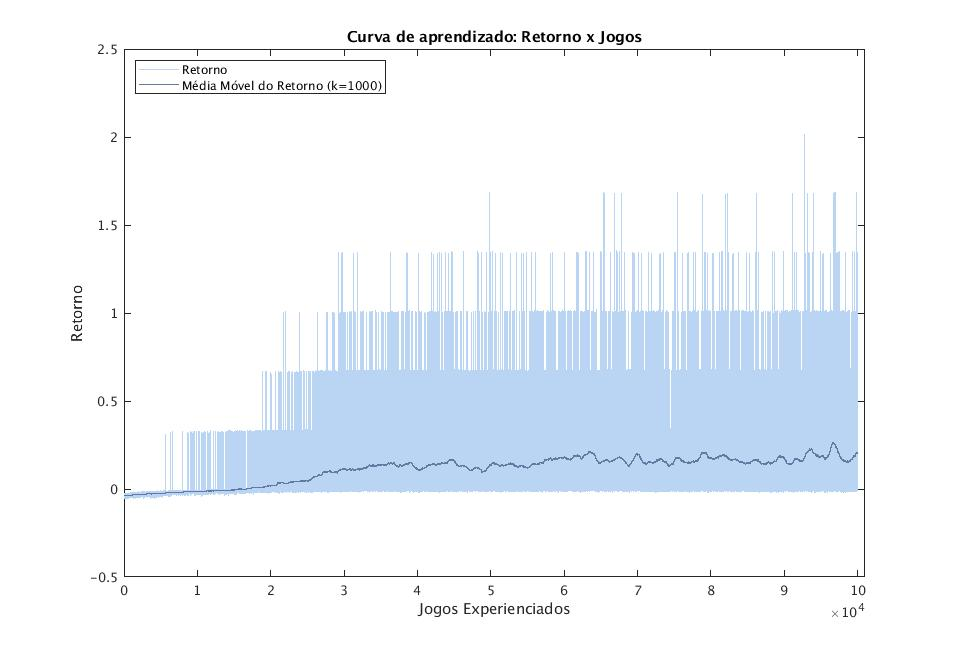
\includegraphics[width=0.8\linewidth]{figs/curva-qtabular.jpg}
	\centering
	\caption{Curva de aprendizado. Para cada jogo foi feita a média entre os 3 retornos observados em cada um dos treinamentos.}
	\label{fig:single-agent-curva}
\end{figure}

Além disso, foi executado um treinamento de 200000 partidas com os mesmos parâmetros, a fim de observar a aprendizagem por um período mais longo.

\begin{figure}[h]
	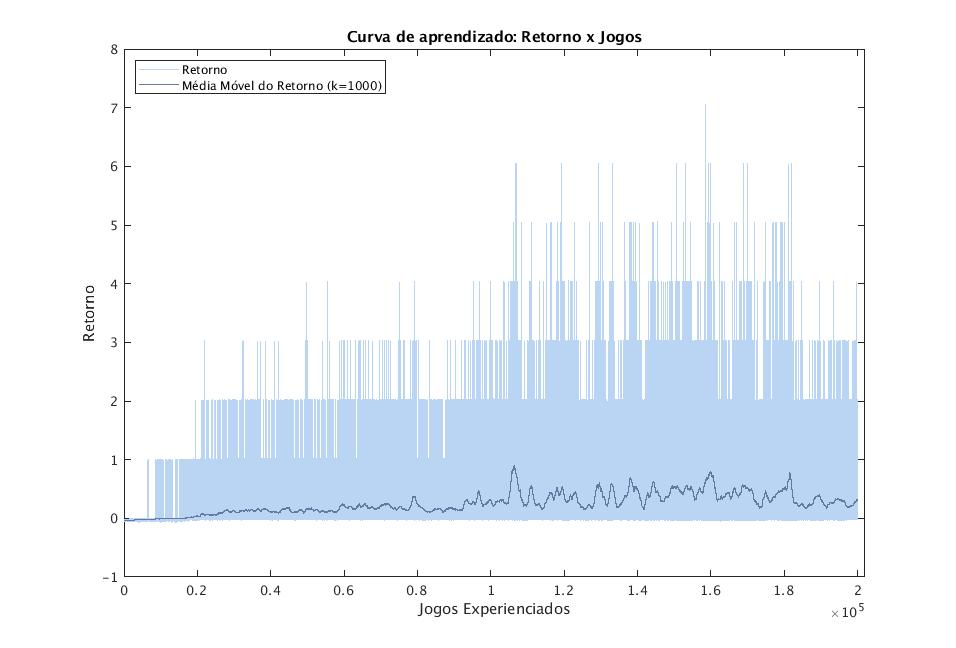
\includegraphics[width=0.8\linewidth]{figs/curvalonga-qtabular.jpg}
	\centering
	\caption{Curva de aprendizado para treinamento longo. Observa-se a cessação de aprendizado com o decaimento do fator de exploração.}
	\label{fig:single-agent-curvalonga}
\end{figure}

Apesar da grande quantidade de experiência a que o agente teve acesso, nota-se que o crescimento de seu desempenho é bastante limitado, sequer atingindo a média de 1 gol por partida. Isso é um indicativo do altíssimo custo computacional de soluções \textit{end-to-end} como a utilizada no experimento.

\section{Agente Único com Double Q-Learning Tabular e Comportamentos Pré-Programados}

% TODO inserir gráficos e comentar resultados do tabular behaviors

% \section{Agentes Concorrentes}

% Após validação do sistema com agente único, é interessante experimentar com treinamento adversarial de apenas 2 jogadores em formato um-contra-um. A intenção dessa etapa é experimentar com o sistema o caso adversarial, no qual há um ou mais agentes com objetivo oposto ao do agente sendo treinado.

% \section{Múltiplos Agentes}

% Após validar os casos de agente único e de agentes concorrentes, propõe-se um treinamento completo em jogos 11 contra 11. O objetivo é, ao final do processo, termos um time capaz de jogar contra os principais times da atualidade na categoria RoboCup Soccer Simulation 2D.

% Para isso, os agentes devem ser capazes de cooperar e reagir aos movimentos da equipe oposta a fim de marcar gols e evitar os gols do adversário.
